\documentclass{ds-report}
\usepackage{float}

\assignment{Java RMI} % Set to `Java RMI`, `Java EE` or `Google App Engine`.
\authorOne{Konstantinos Stefanidis Vozikis} % Name of first team partner.
\studentnumberOne{r0776192} % Student number of first team partner.
\authorTwo{Sofie Landuyt} % Name of second team partner.
\studentnumberTwo{r0665451}  % Student number of second team partner.

\begin{document}
	\maketitle

	\paragraph{How would a client complete one full cycle of the booking process, for both a successful and
failed case? Base yourself on the example scenarios in Figure 1. Create sequence drawings to
illustrate this.\\} 
There are two sequence diagrams. The first one, see Figure 1, displays a successful scenario. The second one, see Figure 2, is a possible outcome of a failed case. The diagram is based on a scenario where the second client tries to rent a specific car that was available at the beginning of the session but while making the reservation some other client rented it first, making the car unavailable.
The two diagrams are also included in the zip-file for extra readability.


	
	\paragraph{When do classes need to be serializable? You may illustrate this with an example class.\\} 
	A class needs to be serializable when an object of that class has to be transferred over a network. To illustrate this, we serialize the CarType class because it is the return type of a method of the ManagerSessionInterface.
	
	\paragraph{When do classes need to be remotely accessible (Remote)? You may illustrate this with  an example class.\\} 
	A class needs to be remotely accessible when certain methods of this class should be available to a client on another machine.
	Our AgencyInterface is remotely accessible, this way the Client class can invoke methods of the CarRentalAgency class that implements AgencyInterface.
	
	\paragraph{What data has to be transmitted between client and server and back when requesting the number
of reservations of a specific renter?\\}
	First, the client has to request new manager session.
	The data that is transmitted here is a ManagerSessionInterface from the Car Rental Agency server to the Client.
	Then, the client name is being transmitted from the client to the same server.
	After this, the Car Rental Agency queries the individual Car Companies. Now, the client name is being transmitted from the Car Rental Agency to every car company.
	The Car Companies each send their result, an integer, to the Car Rental Agency and then the Car Rental Agency sends the total result to the Client.
	
	
	\paragraph{What is the reasoning behind your distribution of remote objects over hosts? Show which
hosts execute which classes, if run in a real distributed deployment (not a lab deployment where everything runs on the same machine). Create a component/deployment diagram to illustrate this: highlight where the client and server are.\\}
	The rental server is responsible for giving the rental agency access to the car companies' information. The client can make reservations through the rental agency.

	
	\paragraph{How have you implemented the naming service, and what role does the built-in RMI registry play? Why did you take this approach?\\}
    The naming service is provided by the CarRentalAgency Class. The class starts naming manager and reservation sessions it provides in the form of
    \[Reservation/ManagerSession\] + a serial id it keeps for both sessions. In that way every session has a unique identifier which is transmitted to
    the client and enables him to lookup the remote object in the registry. The built-in RMI registry binds the objects with the identifier the CarRentalAgency
    indicates on the server side and then is used to lookup the objects using the same identifier on the client side.\\
    This approach was adopted in order to make the application more distributed and more lightweight. By not serializing the whole sessions and passing them
    to the client we achieved a more lightweight approach and for that reason the naming service had to be implemented on the basis of
    passing identifiers over the network so the clients can retrieve the remote objects on their side.
	
	\paragraph{Which approach did you take to achieve life cycle management of sessions? Indicate why you picked this approach, in particular where you store the sessions.\\}
    When a session is created, it is exported on a specified RMI port and its id is bound on the registry. The objects live in the server side
    and the CarRentalAgency class also keeps an index of the created sessions. When a client closes the session, the CarRentalAgency method responsible,
    unbinds the name from the RMI registry and then unexports the object. Afterwards it removes the session from its internal index.
    Since no remote or local reference to the object exists anymore, the object will be destroyed on the next garbage collection.
	
		
	\paragraph{Why is a Java RMI application not thread-safe by default? How does your application of synchronization achieve thread-safety?\\}
    RMI specification does not give any guarantees about different invokations to the same object being executed on the same or different threads
    thus it is not thread-safe by default (https://docs.oracle.com/javase/8/docs/platform/rmi/spec/rmi-arch3.html). \\
    On our application, thread safety is achieved by enforcing synchronization in the appropriate parts of the code. More specifically, to avoid
    naming inconsistencies we block the access to the critical section of the id retrieval and incrementing the serialId of the manager and reservations sessions.
    That way, every id that is produced is unique and no two different objects will be bound to the same id in the registry.
    Also synchronization is implemented in the confirmQuote method of the individual CarRentalCompanies. As a design choice we adopted
    the synchronization only on the level of each individual company rather than the agency. This will be discussed on the next paragraph.

	\paragraph{How does your solution to concurrency control affect the scalability of your design? Could synchronization become a bottleneck?\\}
    Currently we adopted synchronization only on the level of confirmQuote method of the CarRentalCompany. This solution allows a
    good scalability because there is no bottleneck caused on the confirmQuotes method of the Agency as it allows concurrent access.
    A drawback of this, is that the confirmation of quotes is happening on a more "chaotic" way and thus, there is a bigger probability
    that confirming the quotes the fail especially if there are many clients and if the number of quotes they want to confirm is large.
    An alternative design we considered, would be to synchronize the confirmation of quotes on the level of the agency itself. This
    would give us a a higher rate of success on the confirmation of quotes but on the other hand it would lead to a bottleneck as
    more clients confirm their quotes.
    On a real life scenario, the choice between the two would have to be based on studying of traffic or discussion with some project
    manager etc.
    
    \begin{figure}[t]
    \centering
    	\caption{Sequence diagram for a succesful case}
	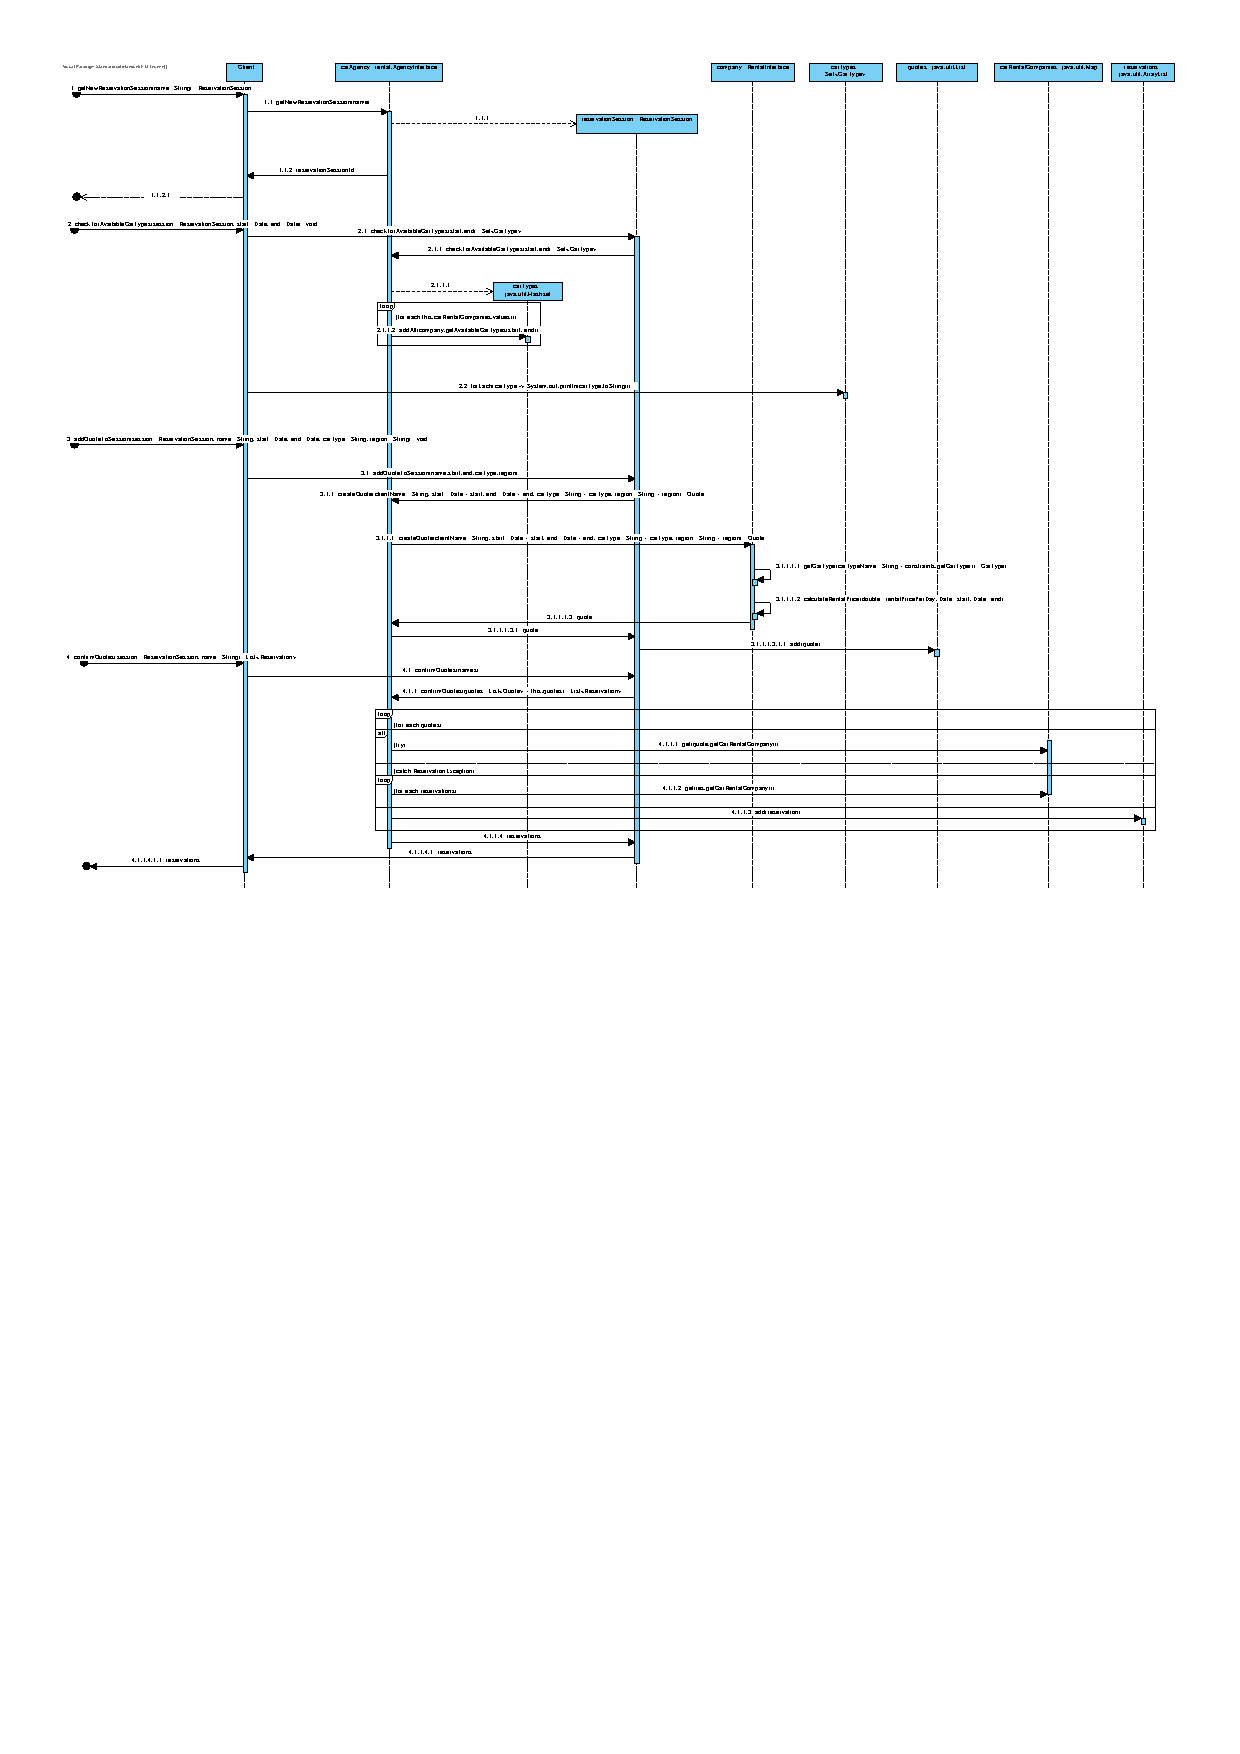
\includegraphics[scale=0.85]{successfulSequenceDiagram}

	\end{figure}
	
	\begin{figure}[t]
		\centering
		\caption{Sequence diagram for a failed case}
	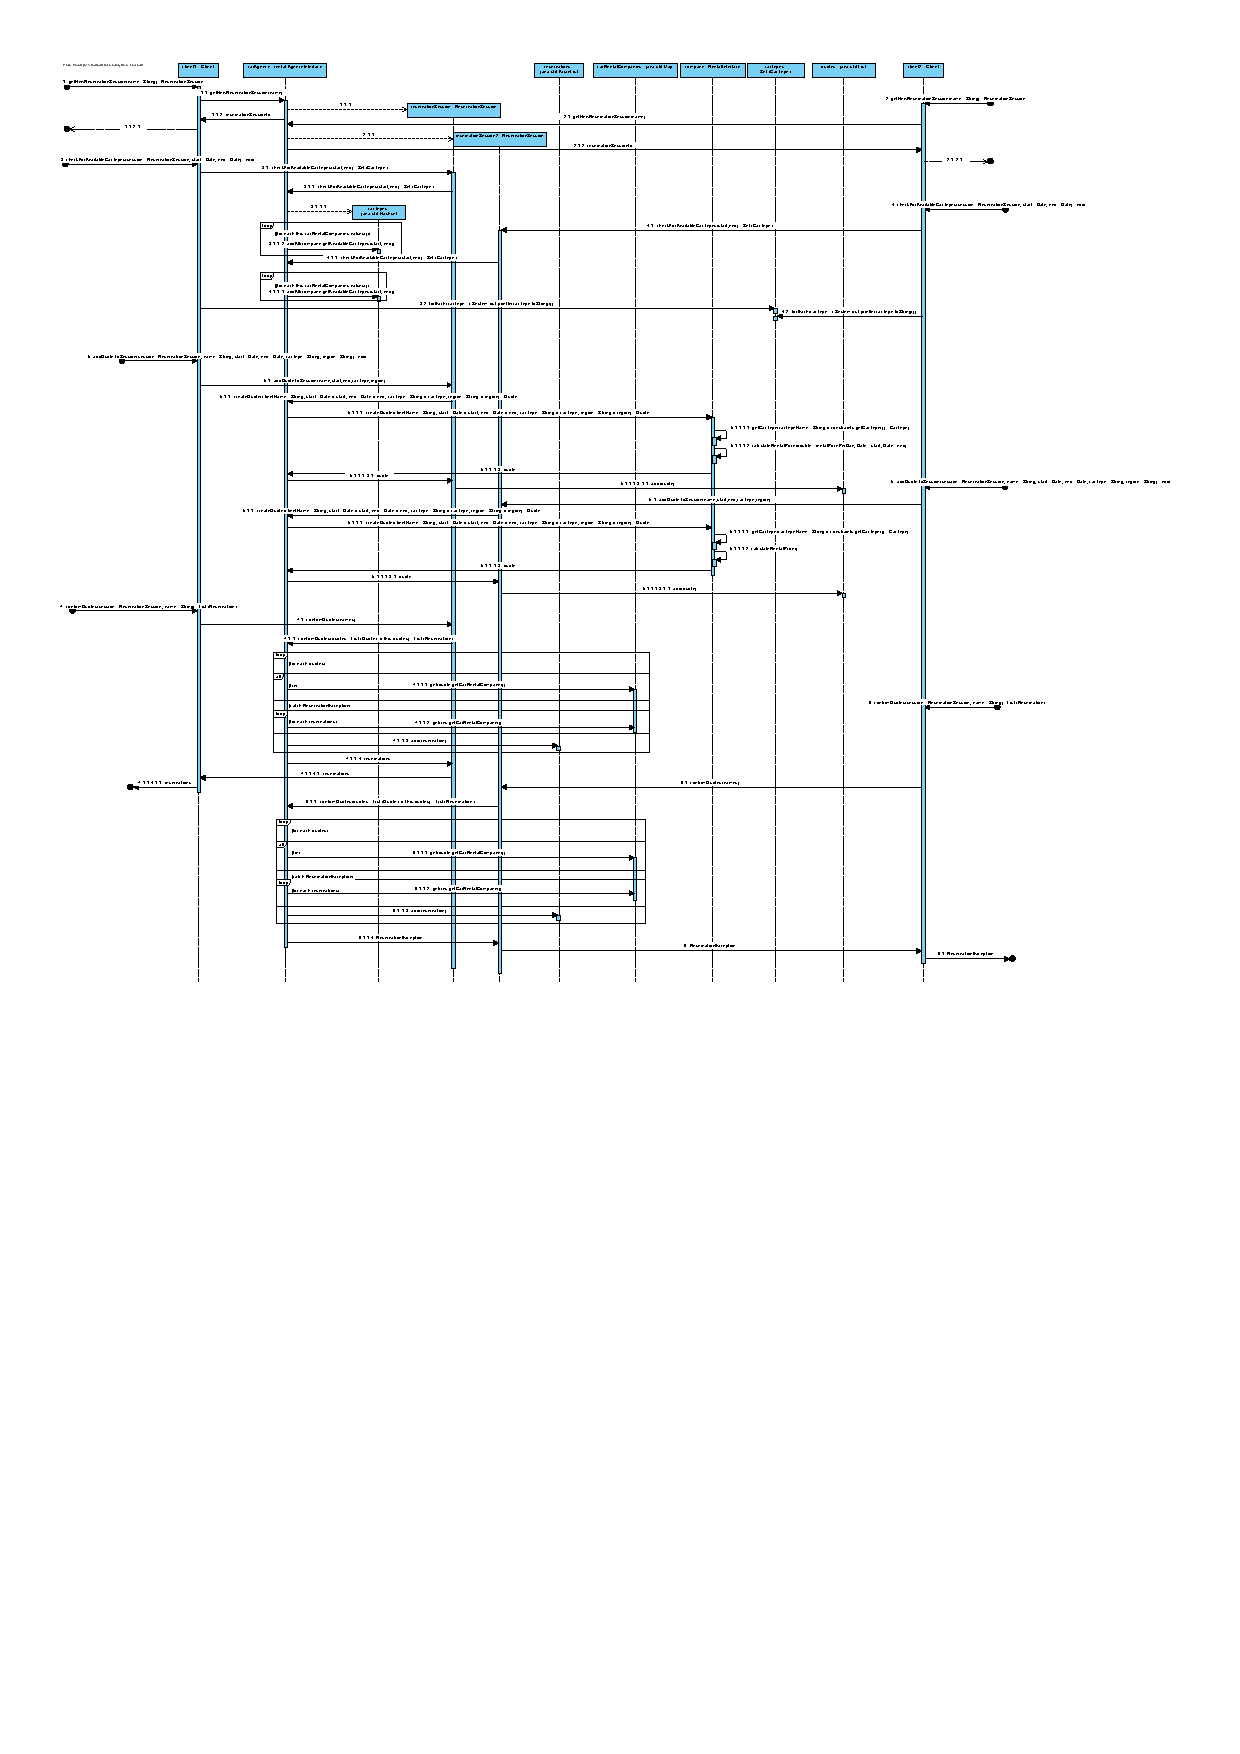
\includegraphics[scale=0.9]{failedSequenceDiagram}
	\end{figure}
	
	\begin{figure}[t]
	\centering
		\caption{Deployment diagram}
	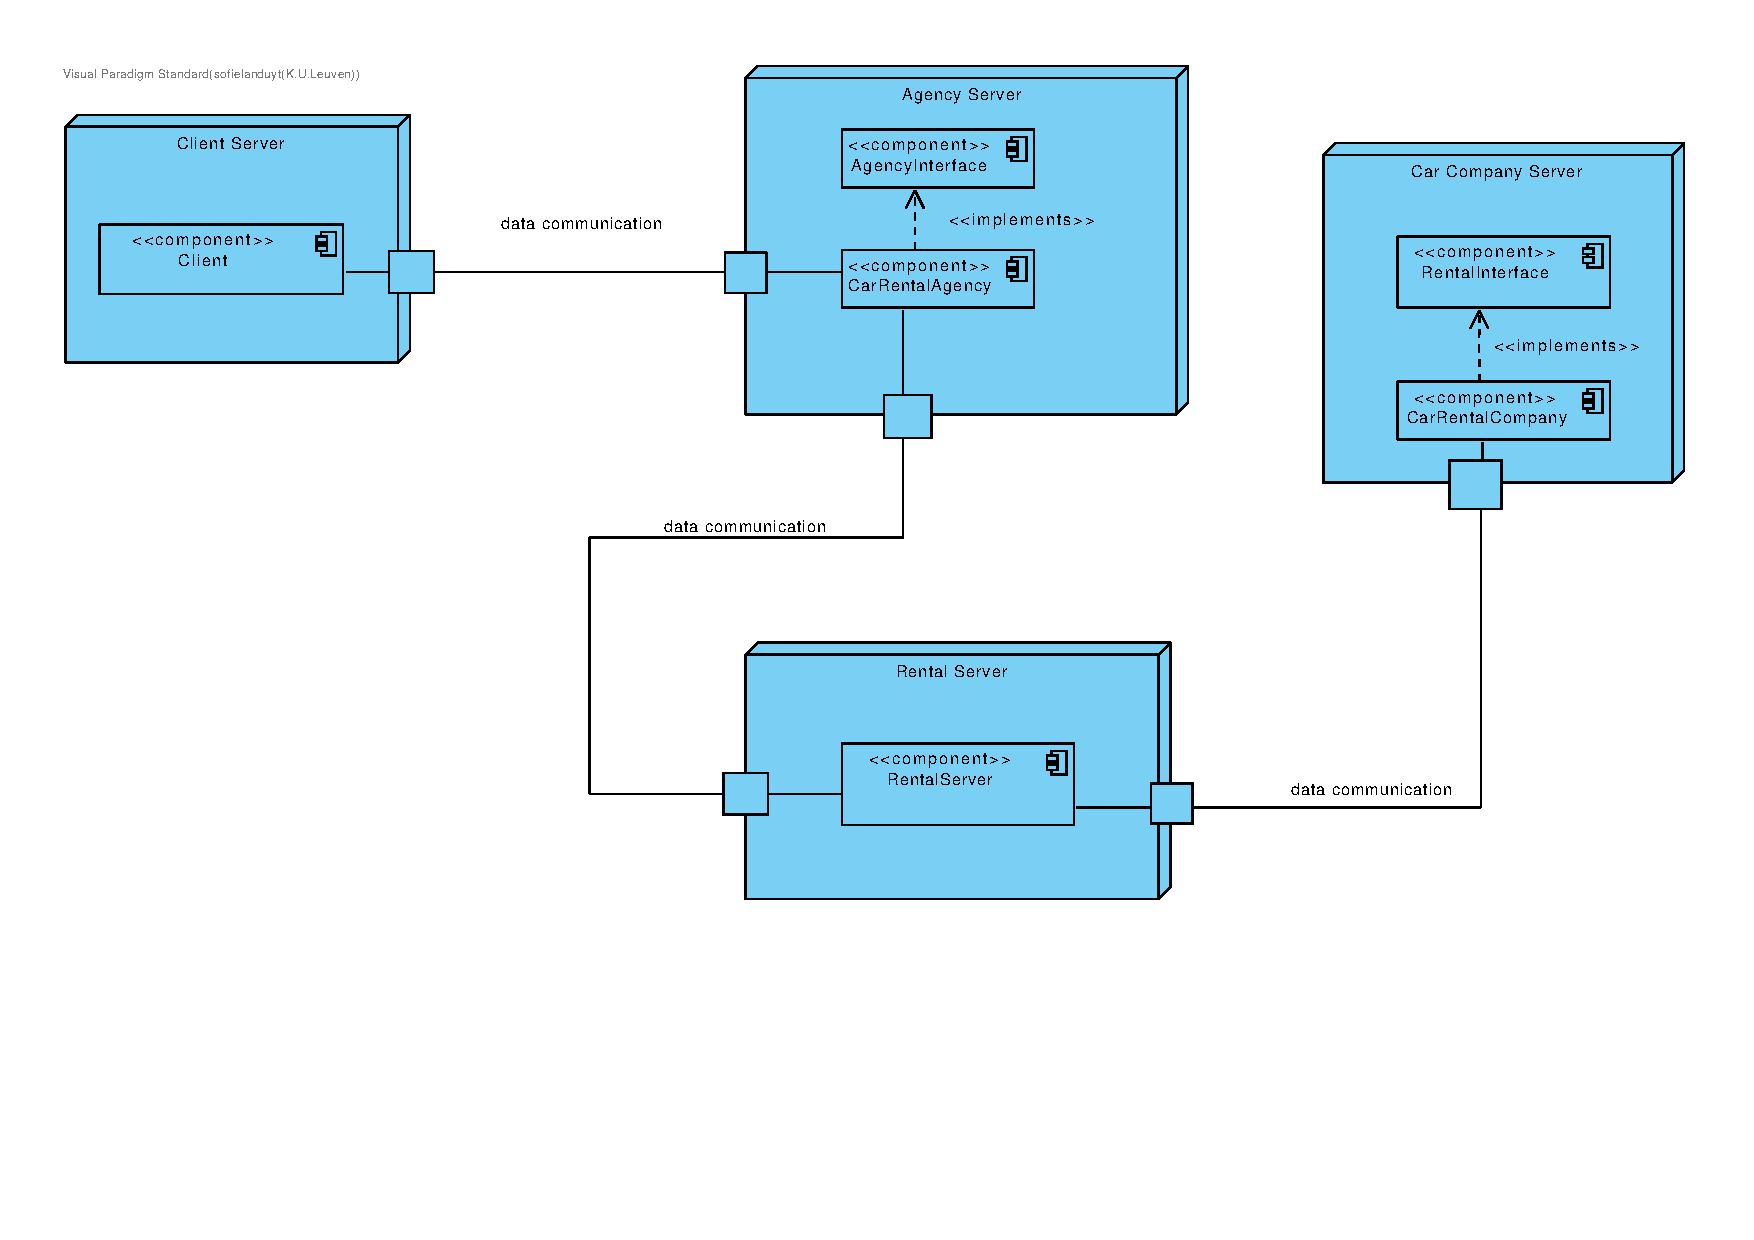
\includegraphics[scale=0.5]{deploymentDiagram}

	\end{figure}	
	
	\clearpage

	
	% You can include diagrams here.
	
\end{document}
